\documentclass[10pt,a4paper]{article}
\usepackage[paper=a4paper, hmargin=1.5cm, bottom=1.5cm, top=3cm]{geometry}

\usepackage[utf8x]{inputenc}
\usepackage[spanish]{babel}

\usepackage{mathtools}
\usepackage{amsmath}
\usepackage{amsfonts}
\usepackage{amssymb}

\usepackage{xcolor}
\usepackage{listingsutf8}
\usepackage{booktabs}
\usepackage{hyperref}
\usepackage{multirow}

\usepackage{caption}
\usepackage{subcaption}

\usepackage{algorithm}
\usepackage{algpseudocode}

\usepackage{graphicx}
\usepackage{tikz}
\usepackage{relsize}
\usepackage{epstopdf}

\DeclarePairedDelimiter{\ceil}{\lceil}{\rceil}

%\let\NombreFuncion=\textsc
%\let\TipoVariable=\texttt

%\newcommand{\TipoFuncion}[3]{%
  %\NombreFuncion{#1}(#2) \ifx#3\empty\else $\to$ \res\,: \TipoVariable{#3}\fi%
%}

% set the default code style
\lstset{
    frame=tb, % draw a frame at the top and bottom of the code block
    tabsize=4, % tab space width
    showstringspaces=false, % don't mark spaces in strings
    numbers=left, % display line numbers on the left
    commentstyle=\color{green}, % comment color
    keywordstyle=\color{blue}, % keyword color
    stringstyle=\color{red} % string color
}

% mathy stuff
\newtheorem{theorem}{Theorem}[section]
\newtheorem{lemma}[theorem]{Lemma}
\newtheorem{proposition}[theorem]{Proposición}
\newtheorem{corollary}[theorem]{Corollary}

\newenvironment{proof}[1][Demostración]{\begin{trivlist}
\item[\hskip \labelsep {\bfseries #1}]}{\end{trivlist}}
\newenvironment{definition}[1][Definición]{\begin{trivlist}
\item[\hskip \labelsep {\bfseries #1}]}{\end{trivlist}}
\newenvironment{example}[1][Example]{\begin{trivlist}
\item[\hskip \labelsep {\bfseries #1}]}{\end{trivlist}}
\newenvironment{remark}[1][Remark]{\begin{trivlist}
\item[\hskip \labelsep {\bfseries #1}]}{\end{trivlist}}

\newcommand{\qed}{\nobreak \ifvmode \relax \else
      \ifdim\lastskip<1.5em \hskip-\lastskip
      \hskip1.5em plus0em minus0.5em \fi \nobreak
      \vrule height0.75em width0.5em depth0.25em\fi}

\title{Investigación Operativa \\ Coloreo Particionado de Grafos}

\newcommand{\order}[1]{$\mathcal{O}(#1)$}

\begin{document}

%% cover page

\maketitle

\bigskip

\begin{table}[h]
\centering
\begin{tabular}{|l l l|}
\hline
Integrante       & \multicolumn{1}{c}{LU}     & Correo electrónico        \\ \hline
Martin Baigorria & \multicolumn{1}{c}{575/14} & martinbaigorria@gmail.com \\ 
Andrés Armesto Brosio & 512/14 & andresarmesto@gmail.com \\  \hline
\end{tabular}
\end{table}

\vfill
\textbf{Resumen:} ???

\textbf{Keywords:} ???

\newpage
\tableofcontents
\newpage

% end cover page

\section{Modelo}

Dado un grafo $G(V,E)$ con $n = |V|$ vertices y $m = |E|$ aristas,  un coloreo de G se define como una asignacion de un color o etiqueta a cada $v \in V$ de forma tal que para todo  par de vertices adyacentes $(p,q) \in E$ poseen colores distintos. El clasico problema de \textit{coloreo de grafos} consiste en encontrar un coloreo del grafo que utilize la menor cantidad de colores posibles.

En este trabajo resolveremos una variante de este problema, el \textit{coloreo particionado de grafos}. A partir de un conjunto de vertices $V$ que se encuentra particionado en $V_1,...,V_k$, el problema consiste en asignar un color $c \in C$ a solo un vertice de cada particion de forma tal que dos vertices adyacentes no reciban el mismo color y minimizando la cantidad de colores utilizados.

Este problema se puede modelar con Programacion Lineal Entera. Para ello, definamos las siguientes variables:

\hspace{1px}

\begin{center}
$x_{pj} = \begin{cases}
  1 & \text{si el color $j$ es asignado al vertice $p$} \\
  0 & \text{en caso contrario}
\end{cases}$

\hspace{1px}

$w_j = \begin{cases}
  1 & \text{si $x_{pj} = 1$ para algun vertice $p$} \\
  0 & \text{en caso contrario}
\end{cases}$
\end{center}

\subsection{Funcion objetivo}

De esta forma la funcion objetivo del LP consiste en minimizar la cantidad de colores utilizados:
\begin{equation}
min \sum_{j \in C} w_j
\end{equation}

Notar que $|C|$ esta acotado superiormente por la cantidad de particiones $k$.

\vspace{10px}

\subsection{Restricciones}

Los vertices adyacentes no comparten color. Recordar que no necesariamente se le asigna un color a todo vertice.
\begin{equation}
x_{ij} + x_{kj} \leq 1 \;\;\;\;\; \forall (i,k) \in E,\;\; \forall j \in C
\end{equation}

Solo se le asigna un color a un unico vertice de cada particion $p \in P$. Esto implica que cada vertice tiene a lo sumo solo un color.
\begin{equation}
\sum_{i \in V_p} \sum_{j \in C} x_{ij} = 1 \;\;\;\;\; \forall p \in P
\end{equation}

Si un nodo usa color $j$, $w_j = 1$:
\begin{equation}
x_{ij} \leq w_j \;\;\;\;\; \forall i \in V, \forall j \in C
\end{equation}

Integralidad y positividad de las variables:
\begin{equation}
x_{ij} \in \{0,1\} \;\;\;\;\; \forall i \in V, \forall j \in C
\end{equation}

\begin{equation}
w_j \in \{0,1\} \;\;\;\;\; \forall j \in C
\end{equation}
\newpage
\section{Branch \& Bound}
La implementación del modelo y del Branch \& Bound se encuentran en el apendice.
\section{Desigualdades}

\subsection{Desigualdad de Clique}

Sea $j_0 \in \{1,...,n\}$ y sea $K$ una clique maximal de $G$. La desigualdad clique están definida por:

\begin{equation}
\sum_{p \in K} x_{pj_0} \leq w_{j_0}
\end{equation}

\begin{proof}
Para esta demostración utilizaremos las desigualdades Chvátal-Gomory sobre las restricciones del LP planteado en la sección \ref{restricciones}, e inducción. A priori, el teorema es bastante intuitivo: si pinto algún vértice de una clique, no puedo pintar ninguno adyacente del mismo color sin importar la forma en la que particione los vértices del grafo. Sea $n$ el tamaño de la clique maximal.

\hfill

\textbf{Casos Base}
\begin{enumerate}
\item $n=1$: Si en la clique maximal tengo sólo un vértice, no existe arista que contenga este vértice, caso contrario la clique tendría al menos dos elementos. Por lo tanto, este vértice puede estar pintado o no dentro de la partición. Es decir, se cumple la ecuación que queremos probar.
\item $n=2$: Si la clique maximal tiene dos elementos, por definición son conexos. Por la restricción que indica que los vértices adyacentes no comparten color, aquí hay 2 opciones. La primera opción es que a ningún vértice se le asigne el color $j_0$. La otra opción es que, dada la estructura de particiones, se le asigne sólo a uno de ellos el color $j_0$. Por lo tanto, vale la desigualdad para $n=2$.
\item $n=3$: Este es el caso más interesante en el que utilizamos la desigualdad de Chvátal-Gomory. Si la clique tiene 3 vértices, hay tres desigualdades que se deben cumplir:

\begin{itemize}
\item $x_{1j_0} + x_{2j_0} \leq 1$
\item $x_{2j_0} + x_{3j_0} \leq 1$
\item $x_{1j_0} + x_{3j_0} \leq 1$
\end{itemize}

\textcolor{red}{Duda:
Multiplicando todas estas desigualdades por $1/2$ y sumando entonces:
$1/2 (x_{1j_0} + x_{2j_0})  + 1/2 (x_{2j_0} + x_{3j_0}) + 1/2 (x_{2j_0} + x_{3j_0}) \leq 3/2$
Desarrollando: $x_{1j_0} + x_{2j_0} +  x_{3j_0} \leq 3/2$.
Como $x_{ij}$ toma valores enteros, se implica:
$x_{1j_0} + x_{2j_0} +  x_{3j_0} \leq 1$
Utilizando la definición de $w_j$ entonces: $x_{1j_0} + x_{2j_0} +  x_{3j_0} \leq w_{j_0}$
Por lo tanto la desigualdad vale para $n=3$.
}

Multiplicando todas estas desigualdades por $1/3$ y sumando entonces:

$1/3 (x_{1j_0} + x_{2j_0})  + 1/3 (x_{2j_0} + x_{3j_0}) + 1/3 (x_{2j_0} + x_{3j_0}) \leq 3/2$

Como $x_{ij}$ toma valores enteros, entonces:
$1/3 (x_{1j_0} + x_{2j_0})  + 1/3 (x_{2j_0} + x_{3j_0}) + 1/3 (x_{2j_0} + x_{3j_0}) \leq 1$

Simplificando: $x_{1j_0} + x_{2j_0} +  x_{3j_0} \leq 1$.

Utilizando la definición de $w_j$ entonces: $x_{1j_0} + x_{2j_0} +  x_{3j_0} \leq w_{j_0}$

Por lo tanto la desigualdad vale para $n=3$.

\end{enumerate}

\hfill

\textbf{Paso Inductivo:} $P(n-1) \implies P(n)$

Como vale la hipótesis inductiva, sabemos que:

\begin{equation*}
\sum_{p \in K-n} x_{pj_0} \leq w_{j_0}
\end{equation*}

\textcolor{red}{
\begin{equation*}
\sum_{p \in K-(n-1)} x_{pj_0} \leq w_{j_0}
\end{equation*}
}

Al agregar un vértice a la clique, agregamos $n-1$ aristas, por lo que deben cumplir:

$x_{1j_0} + x_{nj_0} \leq 1$, $x_{2j_0} + x_{nj_0} \leq 1$,...,
$x_{(n-1)j_0} + x_{nj_0} \leq 1$

Utilizando esto, podemos ver que:

\begin{equation*}
x_{nj_0} + \sum_{p \in K-(n-1)} x_{pj_0} \leq w_{j_0}
\end{equation*}

Esto es claramente equivalente a lo que queremos demostrar y se puede justificar a partir de dos casos:

\begin{itemize}
\item Si al vértice $x_{nj_0}$ se le asigna el color $j_0$, las restricciones de las aristas agregadas agregamos hacen que al resto de los vértices de la clique no se le puede asignar el color $j_0$.
\item Si al vértice $x_{nj_0}$ no se le asigna color, o se le asigna un color diferente a $j_0$, se obtiene la expresión de la hipótesis inductiva, y sabemos que lo que queremos probar vale. \hfill $\square$
\end{itemize}
\end{proof}

\subsection{Desigualdad de Agujero Impar}

Sea $j_0 \in \{1,...,n\}$ y sea $C_{2k+1} = v_1,...,v_{2k+1}$, $k \geq 2$, un agujero de longitud impar. La desigualdad esta definida por:

\begin{equation}
\sum_{p \in C_{2k+1}} x_{pj_0} \leq k w_{j_0}
\end{equation}

\begin{proof}
Por teoremas de coloreo (que se prueban en general por inducción), sabemos que el número cromático $\chi(C) = 3$. En el peor de los casos, cada vértice del agujero estará en una partición diferente. Aquí nuevamente tenemos dos casos:

\begin{itemize}
\item Si no se asigna el color $j_0$ a algún vértice del agujero, la desigualdad vale.
\item Si se asigna el color $j_0$, en el peor de los casos el coloreo particionado coincide con el coloreo tradicional. En ese caso, se asignará el color $j_0$ a lo sumo a $(|C|-1)/2$ vértices. Dado $|C| = 2k+1$,  $(2k+1-1)/2 = k$. Por lo tanto vale la desigualdad.  \hfill $\square$
\end{itemize}

\end{proof}

\subsection{Planos de Corte}

Los algoritmos de planos de corte comenzaron a estudiarse en los años 60's. Fueron introducidos por Ralph E. Gomory, a quien luego se le sumó Václav Schvátal. En sus términos básicos, en un primer paso se resuelve la relajación lineal del problema, es decir aquella que relaja las condiciones de integralidad sobre las variables. Luego, el procedimiento termina si se verifica que el problema es infactible, o si se halla una solución que cumple las condicioens de integralidad. En caso de que no ocurra esto, los \textit{algoritmos de separación} buscan identificar desigualdades lineales que permitan separar el óptimo fraccionario hallado de los puntos enteros factibles. De este modo, se intenta que el poliedro se parezca más a la cápsula convexa. Se dice que la solución fraccionaria \textit{viola} la desigualdad hallada, y al buscarla se debe garantizar que no queden puntos enteros factibles fuera del nuevo poliedro. A continuación, se vuelve a resolver la relajación lineal, agregando en la formulación la desigualdad encontrada. Se repite el proceso hasta que se encuentre una solución que cumpla con la integralidad de las variables, el problema resulte infactible, o no se pueda obtener desigualdades válidas.

Existen algoritmos de separación exactos y heurísticos. Los algoritmos heurísticos, luego de resolver la relajación del problema entero y encontrar una solución óptima $x^*$, retornan una o más desigualdades de la clase violadas la solución $x^*$.

Debido a la naturaleza heurística del algoritmo, es posible que exista una desigualdad de la clase violada, aunque éste sea incapaz de encontrarla. Si se encuentra una desigualdad que es violada por la solución óptima de la relajación, se agrega esta nueva restricción y se vuelve a resolver el programa lineal. Este procedimiento se conoce como algoritmo de plano de corte. Si una solución óptima al problema existe, este tipo de algoritmo no necesariamente la encuentra. Por ejemplo, las heurísticas que encuentran desigualdades válidas pueden fallar, y el algoritmo no puede continuar.

\subsection{Heurísticas}

En general, construir las familias de desigualdades enunciadas en las secciones anteriores de forma exhaustiva es un problema NP-Hard. Por esta razón, los algoritmos heurísticos son sumamente útiles para buscar una aproximación polinomial al problema. Las heurísticas que enunciaremos a continuación utilizan algunas propiedades de la representación de nuestro grafo, ya sea para su construcción o para lograr una mejor complejidad temporal y espacial.

En primer lugar, representamos la estructura del grafo mediante una matriz de adyacencias. Esta matriz se implemento utilizando una lista. Dado que la matriz de adyacencias es simétrica, y la diagonal no es necesaria para este problema en particular, guardamos sólo la parte triangular superior de la misma. Esto nos da la ventaja de poder saber si dos vértices son adyacentes o no en \order{1}, y asimismo reduce la complejidad espacial de forma considerable. La fórmula que utilizamos para generar la biyección entre arista e índice en la lista puede verse claramente en el código. La idea es bastante simple y se basa principalmente en usar la expresión para la suma de enteros consecutivos.

En segundo lugar, numeramos todos los vértices con enteros comenzando con $id = 1$. Por construcción, luego nuestras heurísticas nos garantizarán que nuestro conjunto de índices que representa a un miembro de una familia está ordenado. Esto es muy ventajoso en el sentido que podemos saber fácilmente si un nuevo potencial miembro de la familia esta contenido dentro de un miembro existente. Por otro lado, tiene una clara desventaja: la familia dependerá de como los vértices son numerados.

En un principio, la estrategia que seguimos fue generar las diferentes familias una vez, y luego verificar en cada iteración si la solución de la relajación violaba alguna desigualdad. Dado que esta estrategia en general no daba resultados muy satisfactorios, luego decidimos generar las familias en función del resultado de la relajación para cada iteración.

Por otro lado, muchas veces nuestra heurística generaba familias de desigualdades violadas muy grandes, y agregar todas terminaba siendo contraproducente. Por lo tanto, decidimos buscar algún criterio para poder determinar cuáles son las mejores desigualdades a agregar, y luego definir un $threshold$ para decidir cuántas agregamos al LP. El criterio que utilizamos es el módulo de la diferencia entre los miembros de la desigualdad, aunque pueden existir otros en función también de la cantidad de variables en la desigualdad. Muchas veces las desigualdades más violadas difieren solamente en pocas variables, por lo que esto también podría ser tenido en cuenta.

\subsubsection{Heurística de Separación para Clique Maximal}

Para esta heurística, lo que hacemos es recorrer en orden los vértices que tienen una solución positiva en la relajación del LP. En primer lugar, tomamos el primer vértice, y luego comenzamos a recorrer la lista hasta que encontramos un vértice adyacente. Lo agregamos al conjunto que representa al miembro de la clique, y seguimos agregando elementos en orden de forma que cumplan la adyacentes con todos los que ya hemos agregado. Una vez recorrida toda la lista, agregamos este conjunto a la familia. Luego comenzamos a generar una nueva familia a partir del segundo vértice, y así sucesivamente. Luego agregamos las mejores $threshold$ desigualdades por score. Este procedimiento se puede ilustrar con el siguiente pseudocódigo:

\begin{algorithm}
\caption{Algoritmo para agregar cliques violadas}
\begin{algorithmic}[1]
\Procedure{generateCliqueFamilly}{$V,E,sol,threshold,lp$}
\State $set<score, set<int>> clique\_familly$
\For {$id \leftarrow 1, |V|$}
	\If {$sol[id] > 0 + \epsilon$}
		\State continue
	\EndIf
	\State $set<int> clique$
	\State clique.insert(id)
	\For {$id2 \leftarrow id + 1, |V|$}
		\If {$sol[id2] > 0 + \epsilon$}
			\State continue
		\EndIf
		\If {clique.adyacentToAll(id2)}
			\State clique.insert(id2)
		\EndIf
	\EndFor
	\If {$\neg clique\_familly.isContained(clique)$}
		\State clique\_familly.insert($<getScore(clique), clique>$)
	\EndIf
\EndFor
\State sortByScore(clique\_familly)
\State addTopCliqueRestrictions(lp, clique\_familly, threshold)
\EndProcedure
\end{algorithmic}
\end{algorithm}

Notar que en la práctica sólo consideramos cliques de tamaño mayor a 2, dado que si no se pisan con las restricciones de adyacencia del LP. A su vez, esta heurística debe ser generalizada para todos los colores, lo que no fue mostrado para facilitar la visualización del algoritmo.

\pagebreak

\subsubsection{Heurística de Separación para Agujero Impar}

Para esta heurística, seguimos un procedimiento similar al anterior. Recorremos los vértices en orden, y los vamos agregando si son adyacentes. Al final, el conjunto de vértices resultante es un camino. Luego, vemos si el ultimo elemento del camino es adyacente al primero, y si el camino tiene longitud impar. Si esto sucede, agregamos el conjunto a la familia. Si no sucede, quitamos el ultimo elemento y verificamos nuevamente la condición hasta que se satisfaga. Finalmente, agregamos las mejores $threshold$ desigualdades por score. Este procedimiento se puede ilustrar con el siguiente pseudocódigo:

\begin{algorithm}
\caption{Algoritmo para agregar agujeros impares violados}
\begin{algorithmic}[1]
\Procedure{generateOddholeFamilly}{$V,E,sol,threshold, lp$}
\State $set<score, set<int>> oddhole\_familly$
\For {$id \leftarrow 1, |V|$}
	\If {$sol[id] > 0 + \epsilon$}
		\State continue
	\EndIf
	\State $set<int> path$
	\State path.insert(id)
	\For {$id2 \leftarrow id + 1, |V|$}
		\If {$sol[id2] > 0 + \epsilon$}
			\State continue
		\EndIf
		\If {isAdyacent(path.end, id2)}
			\State path.insert(id2)
		\EndIf
	\EndFor
	\While {path.size() $\geq$ 3 \textbf{and} (path.size() mod 2 == 0 \textbf{or} $\neg$isAdyacent(path.start, path.end))}
		\State path.erase(path.end)
	\EndWhile
	\If {path.size() $\geq$ 3 \textbf{and} isAdyacent(path.start, path.end)}
		\State oddhole\_familly.insert($<getScore(path), path>$)
	\EndIf
\EndFor
\State sortByScore(oddhole\_familly)
\State addTopPathRestrictions(lp, oddhole\_familly, threshold)

\EndProcedure
\end{algorithmic}
\end{algorithm}

Notar que en ambas heurísticas utilizamos la tolerancia $\epsilon$ para evitar problemas numéricos.

\subsection{Cut \& Branch}

Dado que las familias de desigualdades anteriormente expuestas no describen de forma exhaustiva la cápsula convexa del problema, los algoritmos de planos de corte no necesariamente convergen. Por esta razón decidimos implementar un algoritmo Cut \& Branch. Los algoritmos Cut \& Branch buscan aplicar planos de corte a la raíz del árbol de enumeración de Branch \& Bound, lo que \textit{potencialmente} puede mejorar el tiempo de ejecución de los problemas al reducir el espacio de búsqueda y permitiendo mejores podas. Una vez aplicados los cortes, se resuelve el problema resultante mediante Branch \& Bound.

En nuestra implementación, los parámetros que deben ser calibrados para este algoritmo son la cantidad de iteraciones y el threshold. Por cada iteración, el algoritmo resuelve la relajación del problema y agrega a lo sumo $threshold$ restricciones de cada tipo.
\newpage
\section{Experimentación}

Dada la cantidad de vértices, los grafos se generan en el formato estándar DIMACS \footnote{Para ver algunos ejemplos del formato: http://mat.gsia.cmu.edu/COLOR/instances.html}. El generador toma como parámetro la densidad del grafo. Dada una clique con esa cantidad de vértices, se elijen vértices al azar hasta que se llega a la densidad deseada. Debido a que estas instancias están diseñadas para coloreo de grafos, asignamos los vértices de forma uniforme en el total de particiones pasado por parámetro a nuestro programa de coloreo particionado.

Por cuestiones de tiempo, cada uno de los experimientos CPLEX fue ejecutado sin límite de cantidad de threads, con un procesador Intel(R) Core(TM) i7-3610QM CPU @ 2.30GHz y 16GB de memoria RAM.

\subsection{Eliminación de simetría}

Al igual que el problema de coloreo de grafos, el problema del coloreo particionado de grafos presenta una gran cantidad de soluciones simétricas. De no romper la simetría del problema, los algoritmos tendrían un espacio de búsqueda mucho mayor, moviéndose por soluciones que, siendo computacionalmente distintas, en la práctica se trata de la misma. Esto afecta el tiempo de ejecución de forma considerable a medida que crece el tamaño del problema. Para romper la simetría en nuestro problema, en la sección \ref{simetria} mostramos cómo utilizamos la clásica condicion de coloreo de que los colores se deben utilizar en orden. Este fenómeno se puede ver en el siguiente gráfico:

\begin{figure}[h]
\centering
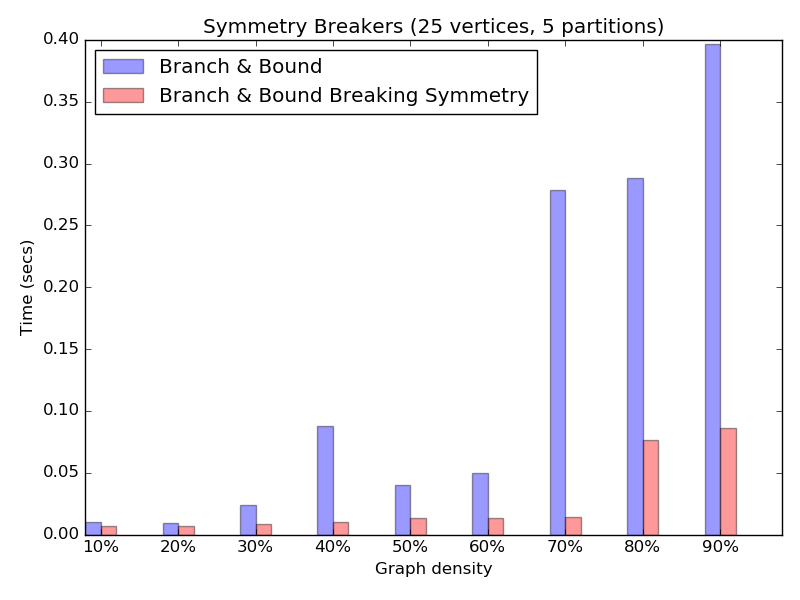
\includegraphics[scale=0.7]{img/2-symmetry_v25_p5_l40_t1_b0.png}
\caption{Tiempo de resolución del modelo incluyendo o no eliminación de simetría.}
\end{figure}

Esto nos brinda la noción sumamente relevante de la importancia y efectividad de romper simetría al realizar la formulación de un LP. Cabe mencionar que existen muchas otras estrategias o expresiones para disminuir aun más el grado de simetría de la formulación. La escogida bajo ninguna circunstancia debe ser considerada la mejor posible.

\pagebreak

\subsection{Efectividad de las familias de desigualdades}

La idea de este experimento es comparar las diferentes estrategias de planos de corte. Para ello, se eligió a 40 como la cantidad de cortes de cada tipo que se podían agregar, con una sola iteración:
% en cada iteración se podían agregar hasta 40 cortes?

\begin{figure}[h]
  \centering
  \begin{minipage}[b]{0.49\textwidth}
    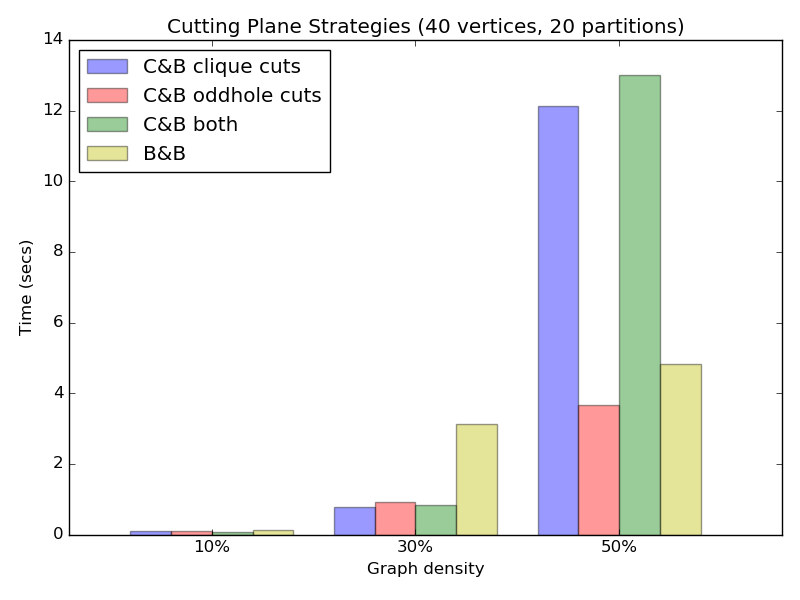
\includegraphics[width=\textwidth]{img/5-cuts_v40_p20_i1_l40_t1_b0.png}
    \caption{Estrategias de planos de corte (tiempo)}
  \end{minipage}
  \hfill
  \begin{minipage}[b]{0.49\textwidth}
    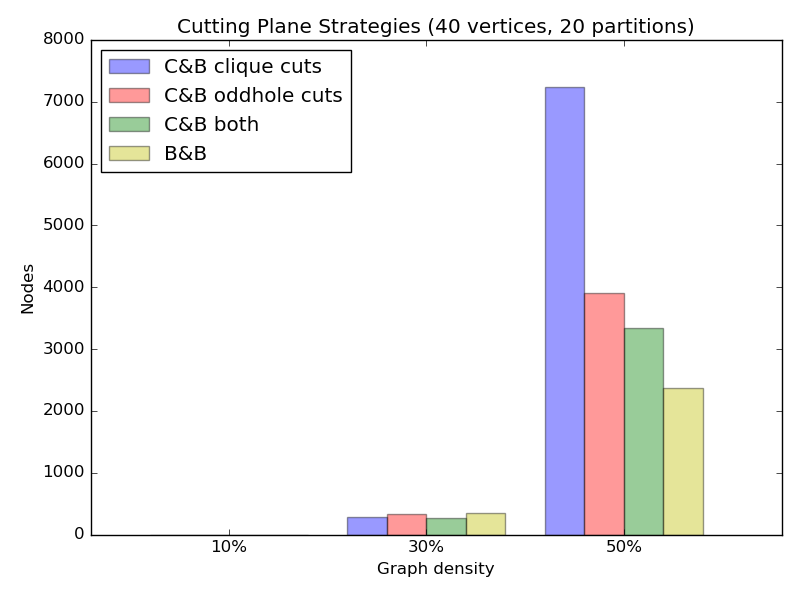
\includegraphics[width=\textwidth]{img/5-cuts_v40_p20_i1_l40_t1_b0_nodes.png}
    \caption{Estrategias de planos de corte (nodos recorridos)}
  \end{minipage}
\end{figure}

Lo primero que podemos observar es que no siempre hay una estrategia ganadora por sobre las otras. Se observa con claridad una dependencia entre la densidad del grafo y la estrategia que tuvo mejores resultados. Cuanto más denso, más cliques nuestra heurística debería encontrar, y a priori uno esperaría que los tiempos mejoren. Esto no sucede, de hecho agregar las restriciones de clique empeora el tiempo de ejecución con respecto al resultado de utilizar B\&B. También podemos observar que un mejor tiempo de ejecución no necesariamente implica que se recorren menos nodos en árbol de enumeración. En contra de lo que esperábamos inicialmente, las desigualdades de agujero impar parecen funcionar bien, aunque por supuesto esto se podría constatar con mayor peso de llevar a cabo una experimentación mas exhaustiva.

\subsection{Efecto de aumentar el número de particiones}

A medida que aumentamos el número de particiones, el problema comienza a parecerse más a uno de coloreo. Dado que las desigualdades que implementamos son clásicas de coloreo, es de esperar que la performance mejore a medida que aumenta el número de particiones \cite{coloring}. Para Cut \& Branch, sólo utilizamos los mejores 40 cortes de clique con una iteración. A medida que aumenta el número de particiones, podemos observar cómo la ganancia del corte es mayor.

\begin{figure}[h]
  \centering
  \begin{minipage}[b]{0.49\textwidth}
    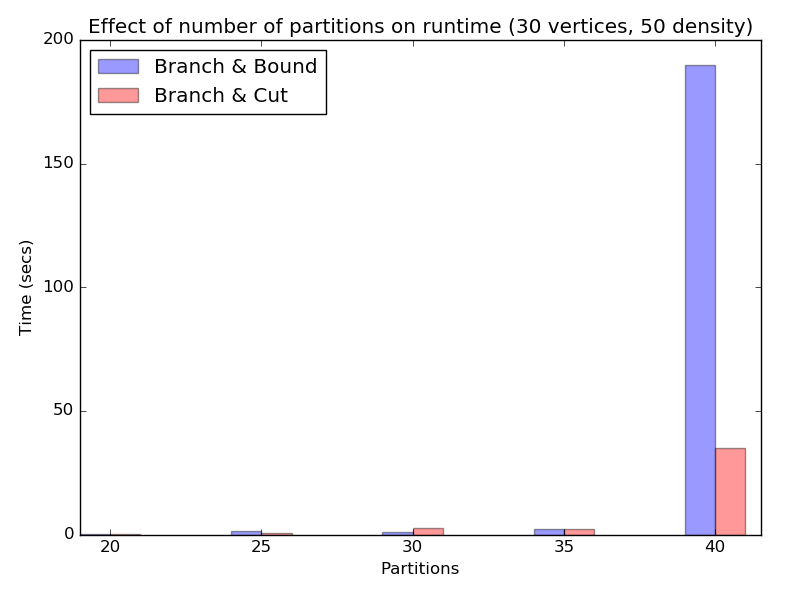
\includegraphics[width=\textwidth]{img/3-partitions_v30_d50_i1_co0_l40_t1_b0.png}
    \caption{Tiempo de ejecucion a medida que aumenta el numero de particiones.}
  \end{minipage}
  \hfill
  \begin{minipage}[b]{0.49\textwidth}
    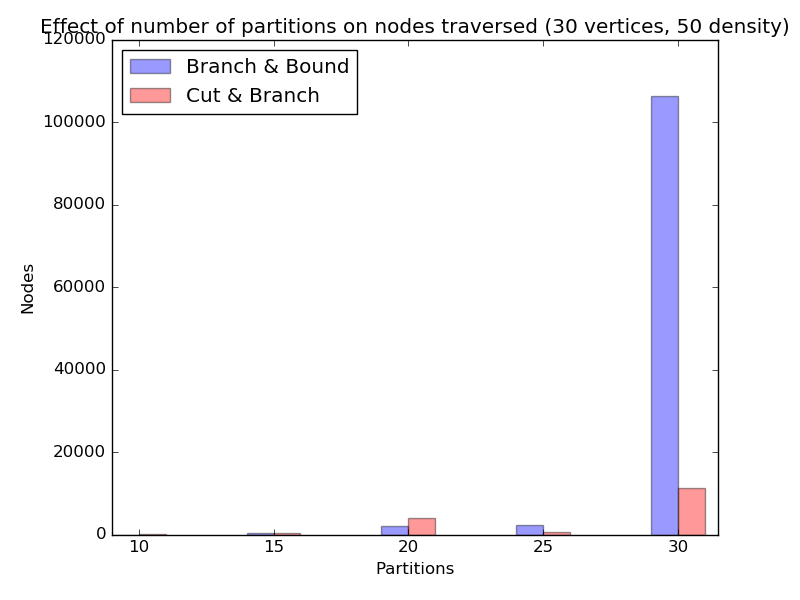
\includegraphics[width=\textwidth]{img/3-partitions_v30_d50_i1_co0_l40_t1_b0_nodes.png}
    \caption{Nodos recorridos a medida que aumenta el numero de particiones.}
  \end{minipage}
\end{figure}

\pagebreak

\subsection{Efecto de aumentar la densidad del grafo}

\begin{figure}[h]
  \centering
  \begin{minipage}[b]{0.49\textwidth}
    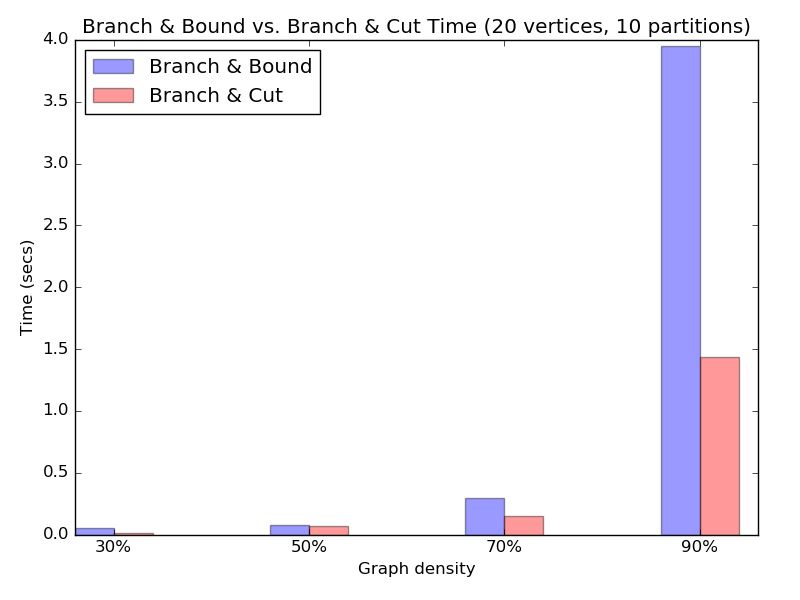
\includegraphics[width=\textwidth]{img/1-bb_vs_bc_v20_p10_i1_co0_l40_t1_b0.png}
  \end{minipage}
  \hfill
  \begin{minipage}[b]{0.49\textwidth}
    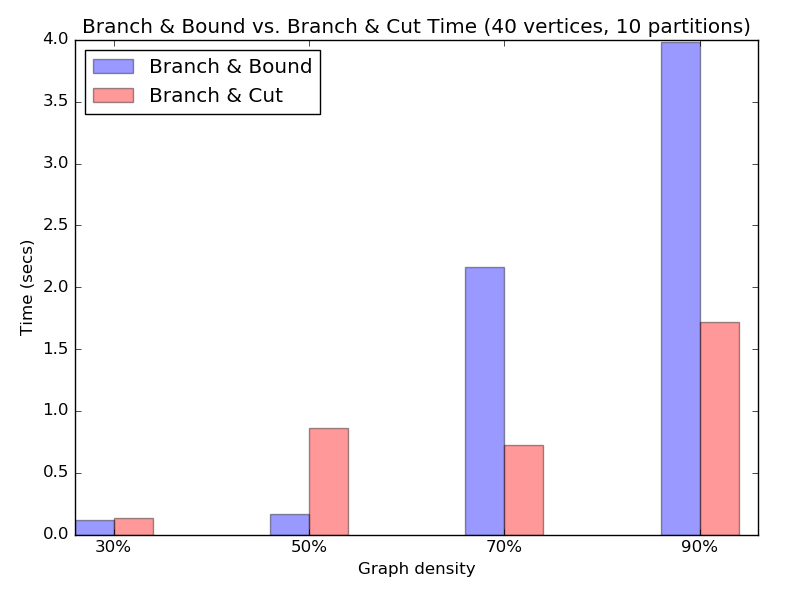
\includegraphics[width=\textwidth]{img/1-bb_vs_bc_v40_p10_i1_co0_l40_t1_b0.png}
  \end{minipage}
  \begin{minipage}[b]{0.49\textwidth}
    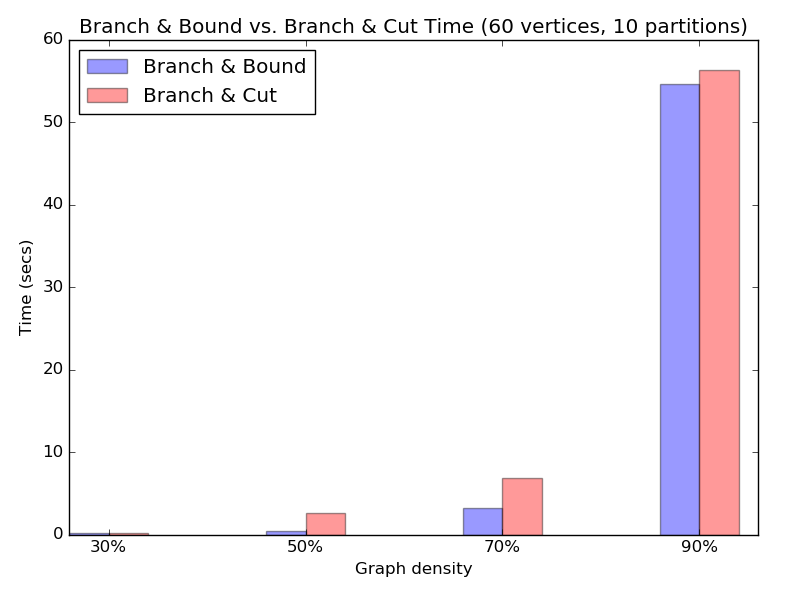
\includegraphics[width=\textwidth]{img/1-bb_vs_bc_v60_p10_i1_co0_l40_t1_b0.png}
  \end{minipage}
  \hfill
  \begin{minipage}[b]{0.49\textwidth}
    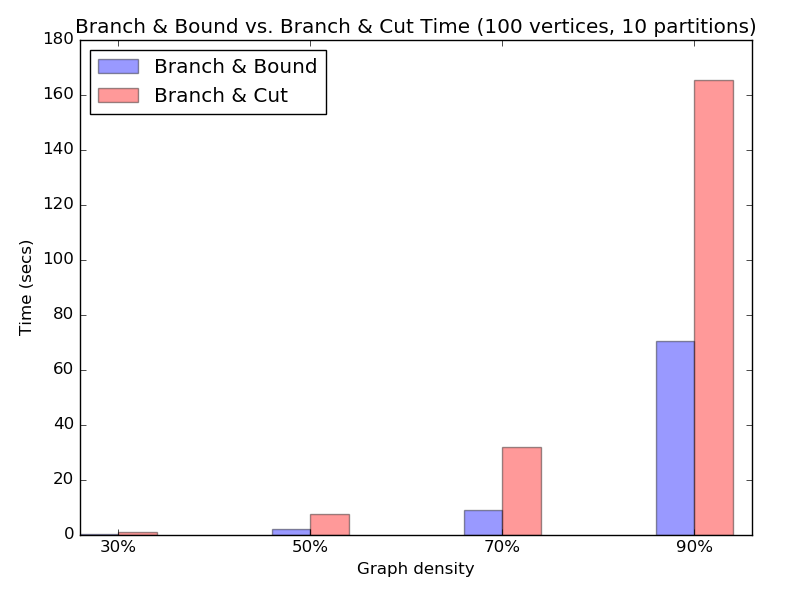
\includegraphics[width=\textwidth]{img/1-bb_vs_bc_v100_p10_i1_co0_l40_t1_b0.png}
  \end{minipage}
	\caption{Efecto de aumentar la densidad del grafo.}
\end{figure}

A medida que aumenta la densidad del grafo, el problema de coloreo se vuelve sin duda más difícil. En los casos donde el número de particiones es mayor en relación al numero de vértices, Branch \& Cut con 1 iteración y 40 desigualdades violadas parece funcionar mejor. Esto no sucede en grafos esparsos, donde Branch \& Bound puro tiene un menor tiempo de ejecución.

\pagebreak

\subsection{Efecto de aumentar la cantidad de restricciones incorporadas por iteración}

Para todos nuestros experimentos en general utilizamos sólo 1 iteración con un límite de 40 desigualdades por familia. La idea de este experimento es evaluar esta configuración. Para ello, utilizamos un grafo con 40 vértices y 20 particiones.

\begin{figure}[h]
  \centering
  \begin{minipage}[b]{0.49\textwidth}
    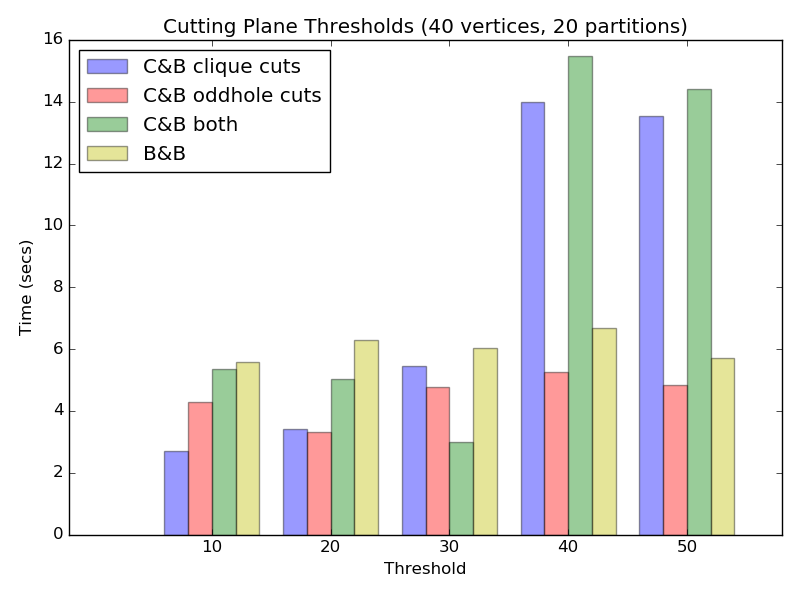
\includegraphics[width=\textwidth]{img/6-thresholds_v40_p20_i1_t1_b0.png}
    \caption{Tiempo de ejecución al incrementar el número de restricciones incorporadas.}
  \end{minipage}
  \hfill
  \begin{minipage}[b]{0.49\textwidth}
    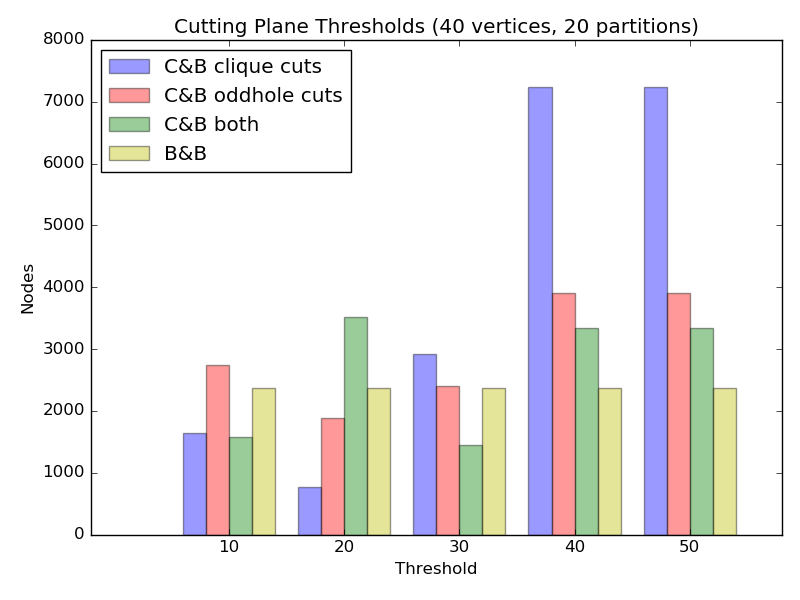
\includegraphics[width=\textwidth]{img/6-thresholds_v40_p20_i1_co2_t1_b0_nodes.png}
    \caption{Nodos recorridos al incrementar el número de restricciones incorporadas.}
  \end{minipage}
\end{figure}

Como podemos observar, agregar más restricciones no es siempre ventajoso. En un principio, agregar restricciones parece mejorar la ejecución del C\&B, pero ya a partir de 40 el tiempo de ejecución empeora de forma abrupta para las cliques. Esto no sucede para las restricciones de agujero impar. Nuevamente, esto se puede deber a que nuestra heurística de clique no es lo suficientemente buena.

\subsection{Efecto de aumentar la cantidad de iteraciones de planos de corte}

\begin{figure}[h]
\centering
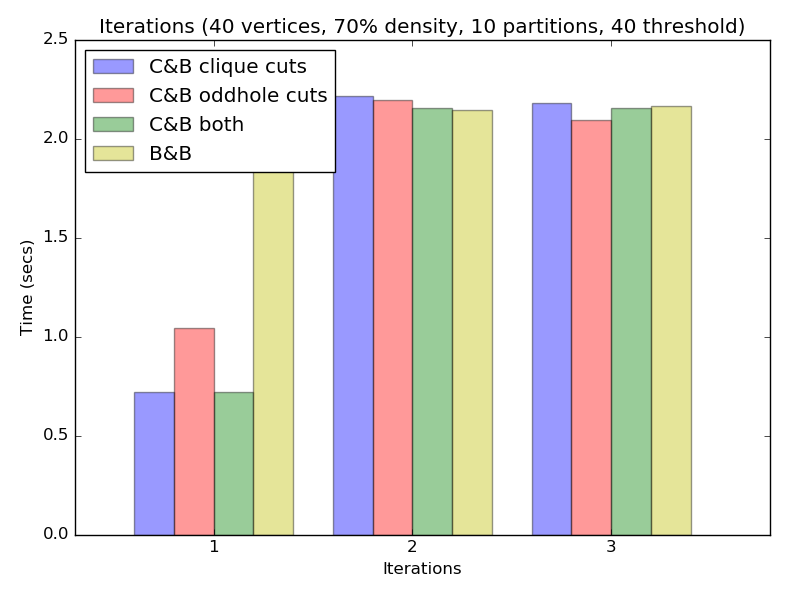
\includegraphics[scale=0.5]{img/7-iterations_v40_p10_l40_t1_b0.png}
\caption{Tiempo de ejecución al aumentar la cantidad de iteraciones de planos de corte.}
\end{figure}

Como podemos ver, aumentar el numero de iteraciones de planos de corte no necesariamente mejora el tiempo de ejecución. En cada iteración lo que hacíamos era generar una familia en función de la solución de la relajación del problema, y luego agregar las \textit{mejores} restricciones. En relación a la sección anterior, esto también esta relacionado con el $threshold$ que elegimos para hacer la experimentación.

\pagebreak

\subsection{Comparación B\&B, C\&B, CPLEX default}

\begin{figure}[h]
  \centering
  \begin{minipage}[b]{0.49\textwidth}
    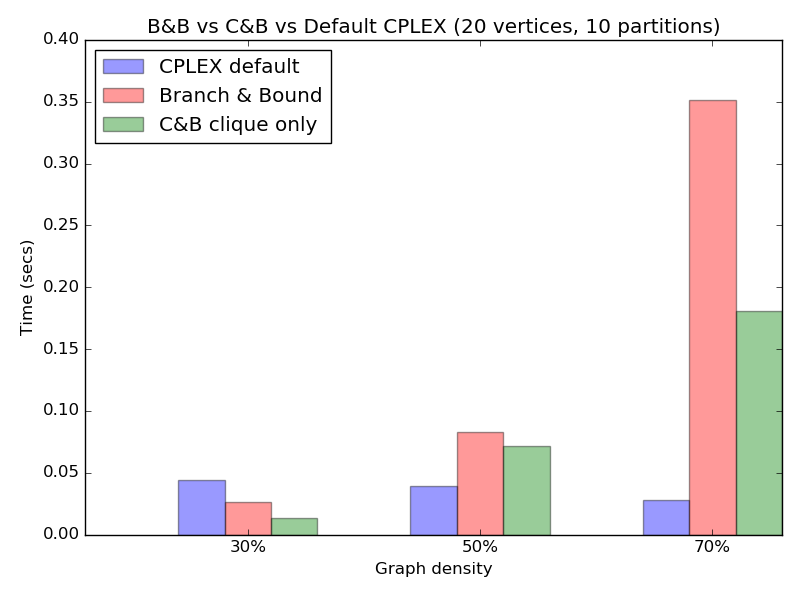
\includegraphics[width=\textwidth]{img/8-compare_v20_p10_i1_l40_t1_b0.png}
  \end{minipage}
  \hfill
  \begin{minipage}[b]{0.49\textwidth}
    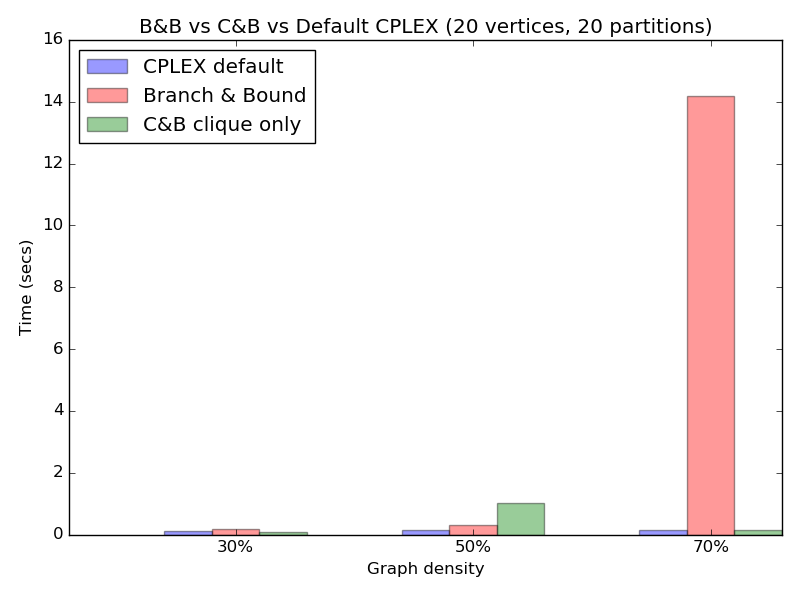
\includegraphics[width=\textwidth]{img/8-compare_v20_p20_i1_l40_t1_b0.png}
  \end{minipage}
  \begin{minipage}[b]{0.49\textwidth}
    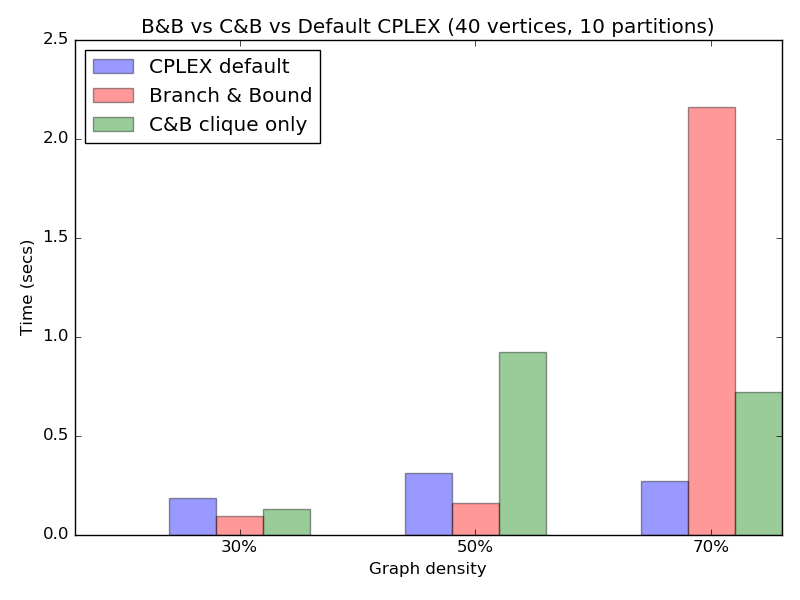
\includegraphics[width=\textwidth]{img/8-compare_v40_p10_i1_l40_t1_b0.png}
  \end{minipage}
  \hfill
  \begin{minipage}[b]{0.49\textwidth}
    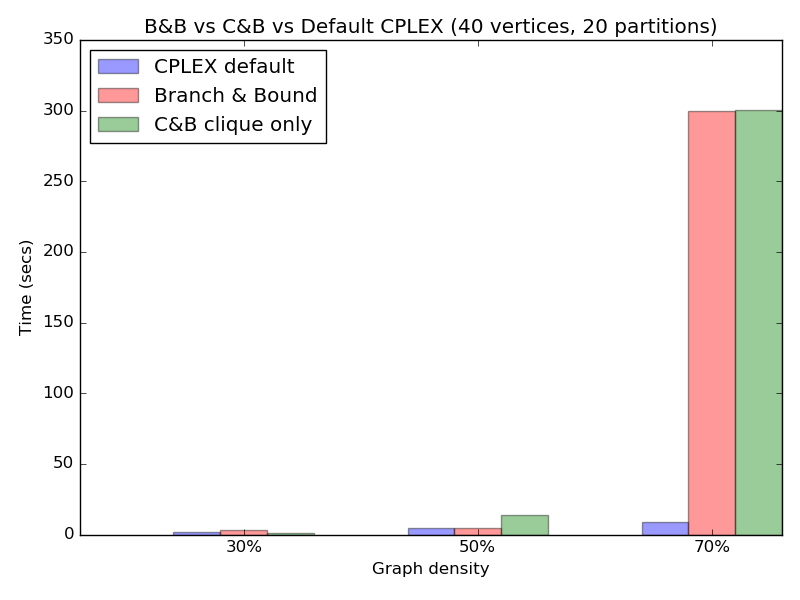
\includegraphics[width=\textwidth]{img/8-compare_v40_p20_i1_l40_t1_b0.png}
  \end{minipage}
	\caption{Comparacion B\&B, C\&B, CPLEX default para diferentes grafos.}
\end{figure}

Dado que el CPLEX por default utiliza cortes de Gomory y preprocesamiento de variables, no nos sorprende que en general sea superior a nuestras otras estrategias para grafos densos. Una propuesta interesante podría ser repetir esta experimentación permitiendo los cortes y el preprocesamiento para todas nuestras estrategias. Otra observación, el gráfico superior derecho es el caso de coloreo de grafos, dado que cada vértice pertenece a una partición diferente. Aquí podemos ver que las desigualdades de clique son sumamente útiles. 

\pagebreak

\subsection{Estrategias de recorrido del árbol de enumeración
y selección de variable de branching}

Existen muchas estrategias de recorrido del árbol de enumeración. En este trabajo solo analizaremos DFS y BBS. DFS (Depth First Search) recorre el árbol de enumeración de B\&B primero en profundidad. Por otro lado, BBS (Best Bound Search) recorre el árbol de enumeración utilizando alguna estrategia para intentar buscar una buena cota lo mas rápido posible. En general se utilizan estrategias heurísticas. En el caso de CPLEX, dado un nodo padre se calcula la solución a la relajación de todos sus hijos y luego se continua recorriendo el nodo con el mayor resultado de la función objetivo. \footnote{http://www-01.ibm.com/support/knowledgecenter/SSSA5P\_12.6.1/ilog.odms.cplex.help/CPLEX/Parameters/topics/NodeSel.html}.

Ambas estrategias son sumamente ventajosas ya que permiten obtener una cota superior a la solución final para utilizar de poda al hacer backtracking sobre el árbol de enumeración. Dado que no utilizamos heurísticas iniciales, esta estrategia parece razonable. 

Por otro lado, las estrategias de selección de variable buscan encontrar cual es la mejor variable sobre la cual hacer branching. Hay muchas reglas, como por ejemplo \textit{max/min infeasibility}. Mientras que la regla de \textit{minimum infeasibility} busca hacer branching sobre mas cercana al entero, la regla de \textit{maximum infeasibility} busca hacer exactamente lo contrario \footnote{http://www-01.ibm.com/support/knowledgecenter/SS9UKU\_12.4.0/com.ibm.cplex.zos.help/Parameters/topics/VarSel.html}.

En esta sección analizaremos 4 combinaciones de estrategias de recorrido del árbol de enumeración y selección de variable de branching para B\&B puro y C\&B con cortes de clique, 1 iteración y $threshold = 30$. Las combinaciones que analizaremos son: DFS + MAXINFEAS, DFS + MININFEAS, BESTBOUND + MAXINFEAS, BESTBOUND + MININFEAS.

\begin{figure}[h]
  \centering
  \begin{minipage}[b]{0.49\textwidth}
    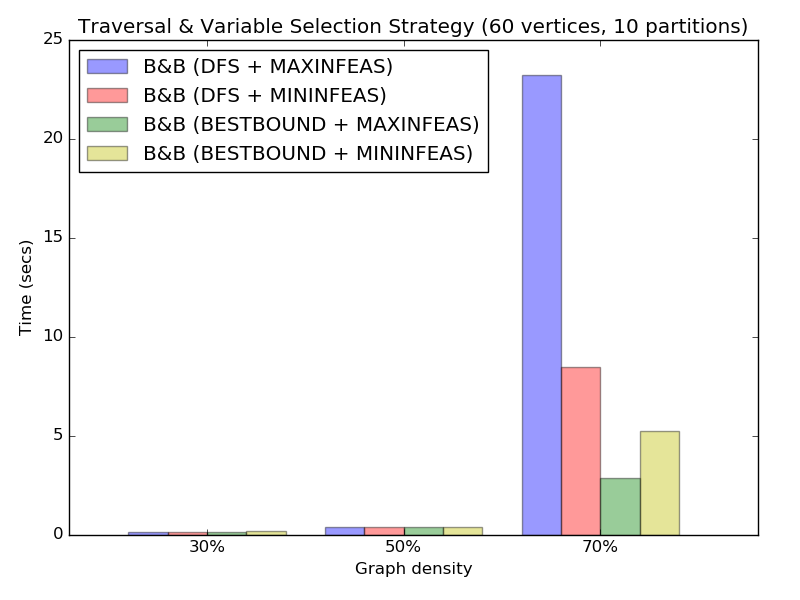
\includegraphics[width=\textwidth]{img/9-tree_v60_p10_i1_l30_s1.png}
  \end{minipage}
  \hfill
  \begin{minipage}[b]{0.49\textwidth}
    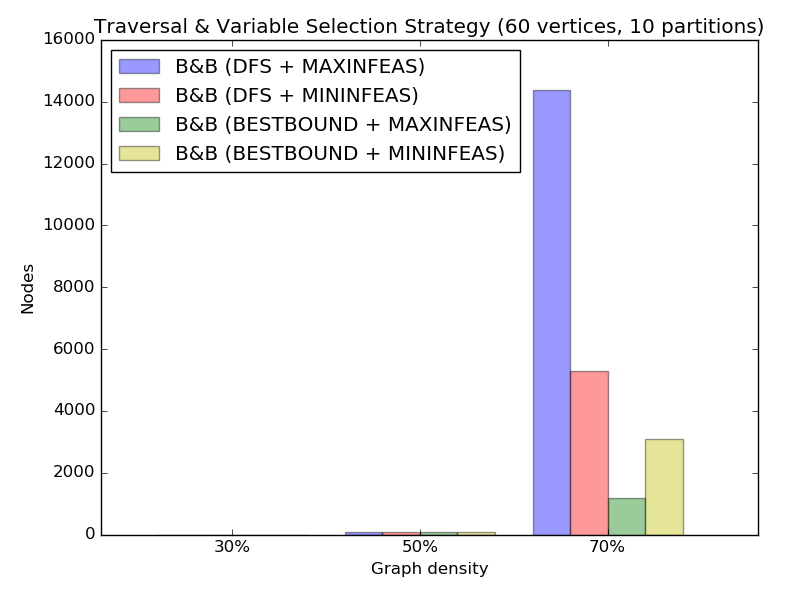
\includegraphics[width=\textwidth]{img/9-tree_v60_p10_i1_l30_s1_nodes.png}
  \end{minipage}
  \begin{minipage}[b]{0.49\textwidth}
    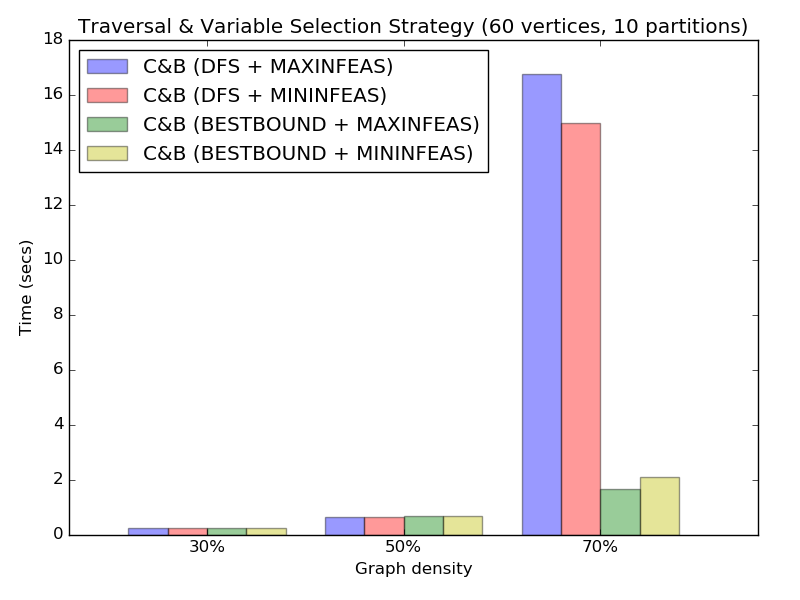
\includegraphics[width=\textwidth]{img/9-tree_v60_p10_i1_l30_s2.png}
  \caption{Tiempo de ejecución dependiendo de la estrategias de recorrido y selección de variable.}
  \end{minipage}
  \hfill
  \begin{minipage}[b]{0.49\textwidth}
    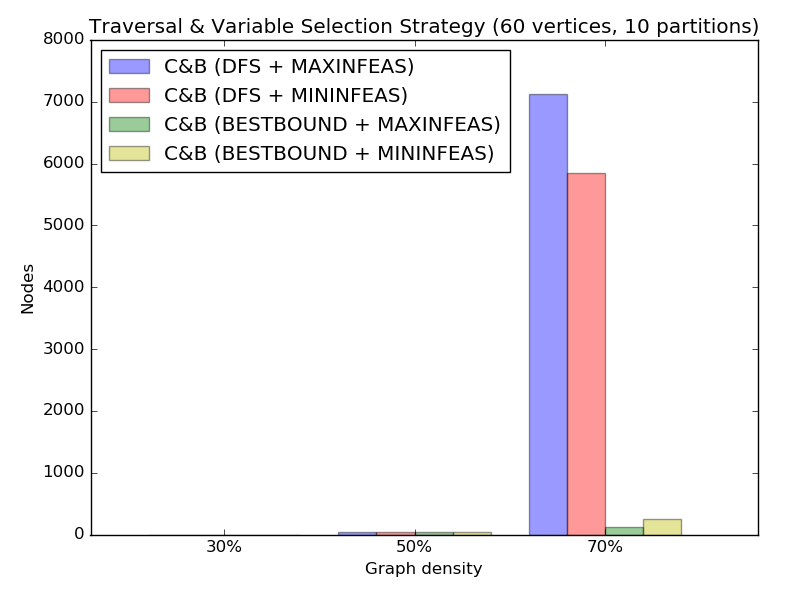
\includegraphics[width=\textwidth]{img/9-tree_v60_p10_i1_l30_s2_nodes.png}
  \caption{Nodos recorridos dependiendo de la estrategias de recorrido y selección de variable.}
  \end{minipage}
\end{figure}

Como podemos observar, en general C\&B tiene tiempos de ejecución menores y a su vez recorre menos nodos. La mejor estrategia para este problema parece ser BESTBOUND + MAXINFEAS. CPLEX utiliza por default BESTBOUND, aunque utiliza una heurística para elegir la variable de branching. 

\subsection{Instancias DIMACS}

Las instancias DIMACS son comúnmente utilizadas en la literatura como instancias de benchmarking. A continuación mostramos nuestros tiempos de ejecución con B\&B y B\&C utilizando 1 iteración y $threshold = 30$ con solo desigualdades de clique. A su vez, ambas utilizan el recorrido del árbol de enumeración dado por default en CPLEX.

Cada tabla utiliza un numero de particiones diferente. Dado que las instancias DIMACS no tienen un numero de partición debido a que se utilizan normalmente para coloreo, asignamos uno nosotros y luego dividimos los vértices en orden en las diferentes particiones de forma uniforme.

Tomamos como tiempo de ejecucion limite 10 minutos, y reportamos el numero de colores encontrado por B\&B hasta ese momento. En todos los casos, B\&B y B\&C coincidieron con el numero de colores utilizados, por lo que los reportamos solo en una columna.

\begin{table}[H]
\centering
\caption{Benchmark con 10 particiones}
\begin{tabular}{|l|r|r|r|r|r|}
\hline
Problem & \multicolumn{1}{l|}{n} & \multicolumn{1}{l|}{m} & \multicolumn{1}{l|}{Tiempo tomado por B\&B (secs)} & \multicolumn{1}{l|}{Tiempo tomado por B\&C (secs)} & \multicolumn{1}{l|}{Colores utilizados} \\ \hline
anna & 138 & 493 & 0.04 & 0.50 & 1 \\ \hline
david & 87 & 406 & 0.02 & 0.29 & 1 \\ \hline
fpsol2.i.1 & 496 & 11654 & 0.51 & 8.71 & 1 \\ \hline
fpsol2.i.2 & 451 & 8691 & 0.44 & 7.66 & 1 \\ \hline
fpsol2.i.3 & 425 & 8688 & 0.45 & 8.15 & 1 \\ \hline
games120 & 120 & 638 & 0.04 & 0.32 & 1 \\ \hline
homer & 561 & 1629 & 0.11 & 0.72 & 1 \\ \hline
huck & 74 & 301 & 0.02 & 0.10 & 1 \\ \hline
inithx.i.1 & 864 & 18707 & 0.79 & 9.66 & 1 \\ \hline
inithx.i.2 & 645 & 13979 & 0.59 & 6.53 & 1 \\ \hline
inithx.i.3 & 621 & 13969 & 0.59 & 6.16 & 1 \\ \hline
jean & 80 & 254 & 0.02 & 0.10 & 1 \\ \hline
le450\_15a & 450 & 8168 & 0.31 & 14.68 & 1 \\ \hline
le450\_15b & 450 & 8169 & 0.35 & 15.68 & 1 \\ \hline
le450\_15c & 450 & 16680 & 0.64 & 36.05 & 1 \\ \hline
le450\_15d & 450 & 16750 & 0.83 & 38.00 & 1 \\ \hline
le450\_25a & 450 & 8260 & 0.34 & 24.95 & 1 \\ \hline
le450\_25b & 450 & 8263 & 0.33 & 15.41 & 1 \\ \hline
le450\_25c & 450 & 17343 & 0.70 & 42.17 & 1 \\ \hline
le450\_25d & 450 & 17425 & 0.70 & 39.60 & 1 \\ \hline
le450\_5a & 450 & 5714 & 0.27 & 8.19 & 1 \\ \hline
le450\_5b & 450 & 5734 & 0.30 & 13.78 & 1 \\ \hline
le450\_5c & 450 & 9803 & 0.46 & 29.12 & 1 \\ \hline
le450\_5d & 450 & 9757 & 0.47 & 33.13 & 1 \\ \hline
miles1000 & 128 & 3216 & 8.81 & 7.77 & 2 \\ \hline
miles1500 & 128 & 5198 & 10 min & 10 min & 3 \\ \hline
miles250 & 128 & 387 & 0.03 & 0.24 & 1 \\ \hline
miles500 & 128 & 1170 & 0.06 & 0.54 & 1 \\ \hline
miles750 & 128 & 2113 & 0.32 & 2.73 & 1 \\ \hline
mulsol.i.1 & 197 & 3925 & 0.15 & 2.20 & 1 \\ \hline
mulsol.i.2 & 188 & 3885 & 0.14 & 2.01 & 1 \\ \hline
mulsol.i.3 & 184 & 3916 & 0.16 & 3.02 & 1 \\ \hline
mulsol.i.4 & 185 & 3946 & 0.15 & 4.37 & 1 \\ \hline
mulsol.i.5 & 186 & 3973 & 0.15 & 3.42 & 1 \\ \hline
myciel2 & 32766 & 0 & 4.37 & 110.76 & 1 \\ \hline
myciel3 & 11 & 20 & 0.01 & 0.01 & 3 \\ \hline
myciel4 & 23 & 71 & 0.01 & 0.02 & 1 \\ \hline
myciel5 & 47 & 236 & 0.01 & 0.04 & 1 \\ \hline
myciel6 & 95 & 755 & 0.04 & 0.29 & 1 \\ \hline
myciel7 & 191 & 2360 & 0.09 & 1.75 & 1 \\ \hline
queen10\_10 & 100 & 1470 & 0.12 & 0.61 & 1 \\ \hline
queen11\_11 & 121 & 1980 & 0.18 & 1.03 & 1 \\ \hline
queen12\_12 & 144 & 2596 & 0.36 & 2.29 & 1 \\ \hline
queen13\_13 & 169 & 3328 & 0.44 & 2.73 & 1 \\ \hline
queen14\_14 & 196 & 4186 & 0.18 & 5.05 & 1 \\ \hline
queen15\_15 & 225 & 5180 & 0.23 & 7.02 & 1 \\ \hline
queen16\_16 & 256 & 6320 & 0.23 & 8.62 & 1 \\ \hline
queen5\_5 & 25 & 160 & 0.06 & 0.14 & 3 \\ \hline
queen6\_6 & 36 & 290 & 0.12 & 0.54 & 2 \\ \hline
queen7\_7 & 49 & 476 & 0.12 & 0.41 & 2 \\ \hline
queen8\_12 & 96 & 1368 & 3.54 & 3.96 & 2 \\ \hline
queen8\_8 & 64 & 728 & 0.26 & 0.64 & 2 \\ \hline
queen9\_9 & 81 & 1056 & 1.76 & 2.54 & 2 \\ \hline
school1 & 385 & 19095 & 1.17 & 90.04 & 1 \\ \hline
school1\_nsh & 352 & 14612 & 0.83 & 46.13 & 1 \\ \hline
zeroin.i.1 & 211 & 4100 & 0.16 & 4.87 & 1 \\ \hline
zeroin.i.2 & 211 & 3541 & 0.17 & 3.82 & 1 \\ \hline
zeroin.i.3 & 206 & 3540 & 0.25 & 1.91 & 1 \\ \hline
\end{tabular}
\end{table}



\newpage
\section{Conclusión}

El famoso problema de coloreo de grafos, que ha sido estudiado ampliamente en la literatura, es un caso particular del coloreo particionado de grafos, donde cada vértice pertenece a una partición diferente. Por esta razón, en primer lugar notamos que el problema del coloreo particionado iba a ser al menos tan difícil como el problema de coloreo, que ya en si es un problema sumamente complicado.

Las desigualdades de planos de cortes que se han implementado en este trabajo son desigualdades utilizadas normalmente para coloreo. Por esta razón, notamos a lo largo de todo el trabajo que en general los algoritmos de Cut \& Branch funcionan bien a medida que aumenta el número de particiones. La intuición nos sugiere que deben existir mejores familias que exploten el hecho de que el grafo esté dividido en particiones, aunque encontrarlas escape del alcance de este trabajo \cite{coloring}.

Uno de los primeros problemas que encontramos al programar el algoritmo de Cut \& Branch fue tener buenas heurísticas para las familias de desigualdades que probamos válidas. Aquí es donde interviene sin duda la creatividad del investigador para diseñar estas heurísticas, principalmente porque se sabe que generarlas de manera exhaustiva es un problema NP-Hard. A lo largo de este trabajo probamos varias estrategias, y finalmente nos quedamos con una que depende de la solución de la relajación en cada iteración. Sin embargo, no tenemos ninguna duda de que existen heurísticas mucho más efectivas. A su vez, una vez encontrado este conjunto de desigualdades violadas, es sumamente importante establecer un criterio para decidir cuáles deben ser agregadas al programa lineal. Se pudo comprobar, en términos generales, que agregarlas todas hace que la optimización sea más lenta.

Por otro lado, en general notamos que el tiempo de cómputo no está dominado por la generación de estas familias, sino por la resolución del programa lineal. Probablemente esto no siempre sea cierto, y el investigador deba procurar un balance entre el tiempo de ejecución de la heurística y el tiempo de ejecución necesario para resolver el programa lineal. Por ejemplo, si consideramos el caso extremo donde generamos la familia entera, este problema es no polinomial, y seguramente dominará el tiempo de ejecución.

A lo largo de este trabajo, la performance de CPLEX nos sorprendió notablemente. Por default, CPLEX en sí funciona bastante bien. Conseguir una mejor descripción de la cápsula convexa muchas veces es muy difícil, y \textit{en términos prácticos} puede llegar a no valer la pena. Debe balancearse el esfuerzo y la dificultad con el tiempo de cómputo y la calidad de la solución obtenido. Por supuesto, también influye el tamaño de instancia que uno necesite resolver. Aquí es donde entra CPLEX, que con una formulación simple del PPL logra optimizar el problema relativamente bien para instancias razonablemente chicas. Como comentario, comprobamos la suma importancia de romper con la simetría de los problemas. Esto en general no representa mucha dificultad, y mejora los tiempos de ejecución de forma considerable.

Una posible mejora para resolver este problema sería implementar un algoritmo Branch \& Cut, buscando buenas heurísticas iniciales y primales para el cálculo de cotas del óptimo, y haciendo cortes en cada nodo del árbol utilizando los \textit{callbacks} de CPLEX \cite{cplex}. Asimismo, podrían incluirse estrategias de preprocesamiento.

Existe gran cantidad de parámetros a calibrar para lograr una buena performance, y su elección en general se basa en una experimentación que logre emular los casos más comunes en la práctica. Durante este trabajo, no se experimentó en profundidad con instancias y problemas sumamente difíciles, debido al tiempo acotado para realizar el mismo. Sería interesante, sin embargo, ver hasta qué punto pueden llegar los algoritmos con una buena configuración.

\section{Apéndice A: Código}
\subsection{coloring.cpp}
\lstinputlisting[language=C++, breaklines=true]{../src/coloring.cpp}
\end{document}